%\documentclass{article}
%\usepackage{graphicx,subfigure}
%\begin{document}

\begin{figure}[!h]
  \centering
   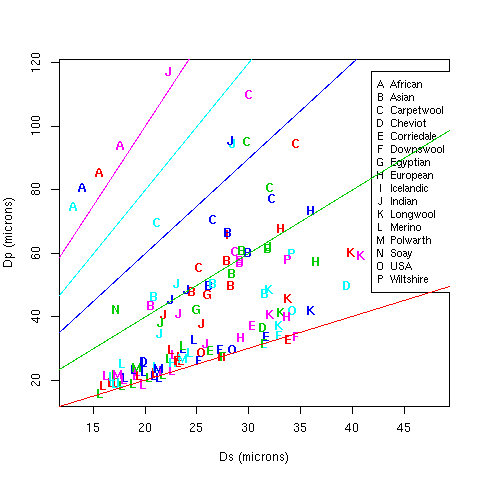
\includegraphics[width=1.0\textwidth]{dsdpalltype.png}
  \caption{Plot of breed means of secondary fibre diameter $D_{s}$ and primary fibre diameter $D_{p}$ for 126 flocks sampled by Carter(1968)~\cite{cart:68}. The breeds have been grouped into a {\em breed type} which in some cases is an individual breed and in other cases is a country of origin. The coloured lines represent various values of the ratio $D_{p}/D_{s}$. Red is $D_{p}/D_{s}=1$, green is $D_{p}/D_{s}=2$, blue is $D_{p}/D_{s}=3$, cyan is $D_{pi}/D_{s}=4$, and magenta is $D_{p}/D_{s}=5$.}
  \label{fig:dsdptype}
\end{figure}

%\end{document}

